\documentclass{article}
\usepackage[utf8]{inputenc}
\usepackage{pgfplots}
\pgfplotsset{width=10cm,compat=1.9}
\usepackage{amsmath,amssymb,amsthm}
\usepackage{graphicx}
\usepackage{float}
\usepackage{blindtext}
\usepackage{hyperref}
\usepackage{verbatim}
\usepackage{gensymb}
\usepackage{enumerate}
\usepackage{xcolor}
\usepackage{graphicx}
\hypersetup{
    colorlinks=true,
    linkcolor=blue,
    filecolor=magenta,      
    urlcolor=cyan,
    pdftitle={Overleaf Example},
    pdfpagemode=FullScreen,
    }
\usepackage[slovene]{babel}

\setlength{\parindent}{0pt}
\setlength{\parskip}{4pt}

\newcounter{example}[section]
\newenvironment{example}[1][]{\refstepcounter{example}\par\medskip
   \noindent \textbf{Naloga~\theexample. #1} \rmfamily}{\medskip}

\newtheorem*{zgled}{Zgled}

\title{Vektorji}
\author{Bor Bregant}
\date{\vspace{-5ex}}

\begin{document}

\maketitle

\section{Vektorji}

Vektor je množica usmerjenih daljic, ki imajo isto velikost in ležijo na vzporednih nosilkah. Operiramo le z enim predstavnikom vektorjev.

Vektorju $\vec{a}=\vec{AB}$ lahko določimo:

\begin{enumerate}[i]
    \item Velikost: $|\vec{AB}|=d(A,B)$
    \item Smer in usmerjenost: Določena s premico nosilko in usmerjenostjo
\end{enumerate}

Vektorja sta enaka, če imata enako velikost, ležita na vzporednih premicah in sta enako usmerjena.

\subsection*{Operacije z vektorji}

\subsubsection*{Seštevanje in odštevanje vektorjev}

Dvočlena operacija, ki dvema vektorjema priredi nov vektor (vsoto). Operacija je komutativna in asociativna.

\begin{enumerate}[i]
    \item Paralelogramsko pravilo - premaknemo vektorja na skupni začetek in vsota je diagonala
    \item Trikotniško pravilo - premikamo na konec naslednjega vektorja
\end{enumerate}

\begin{figure}[H]
    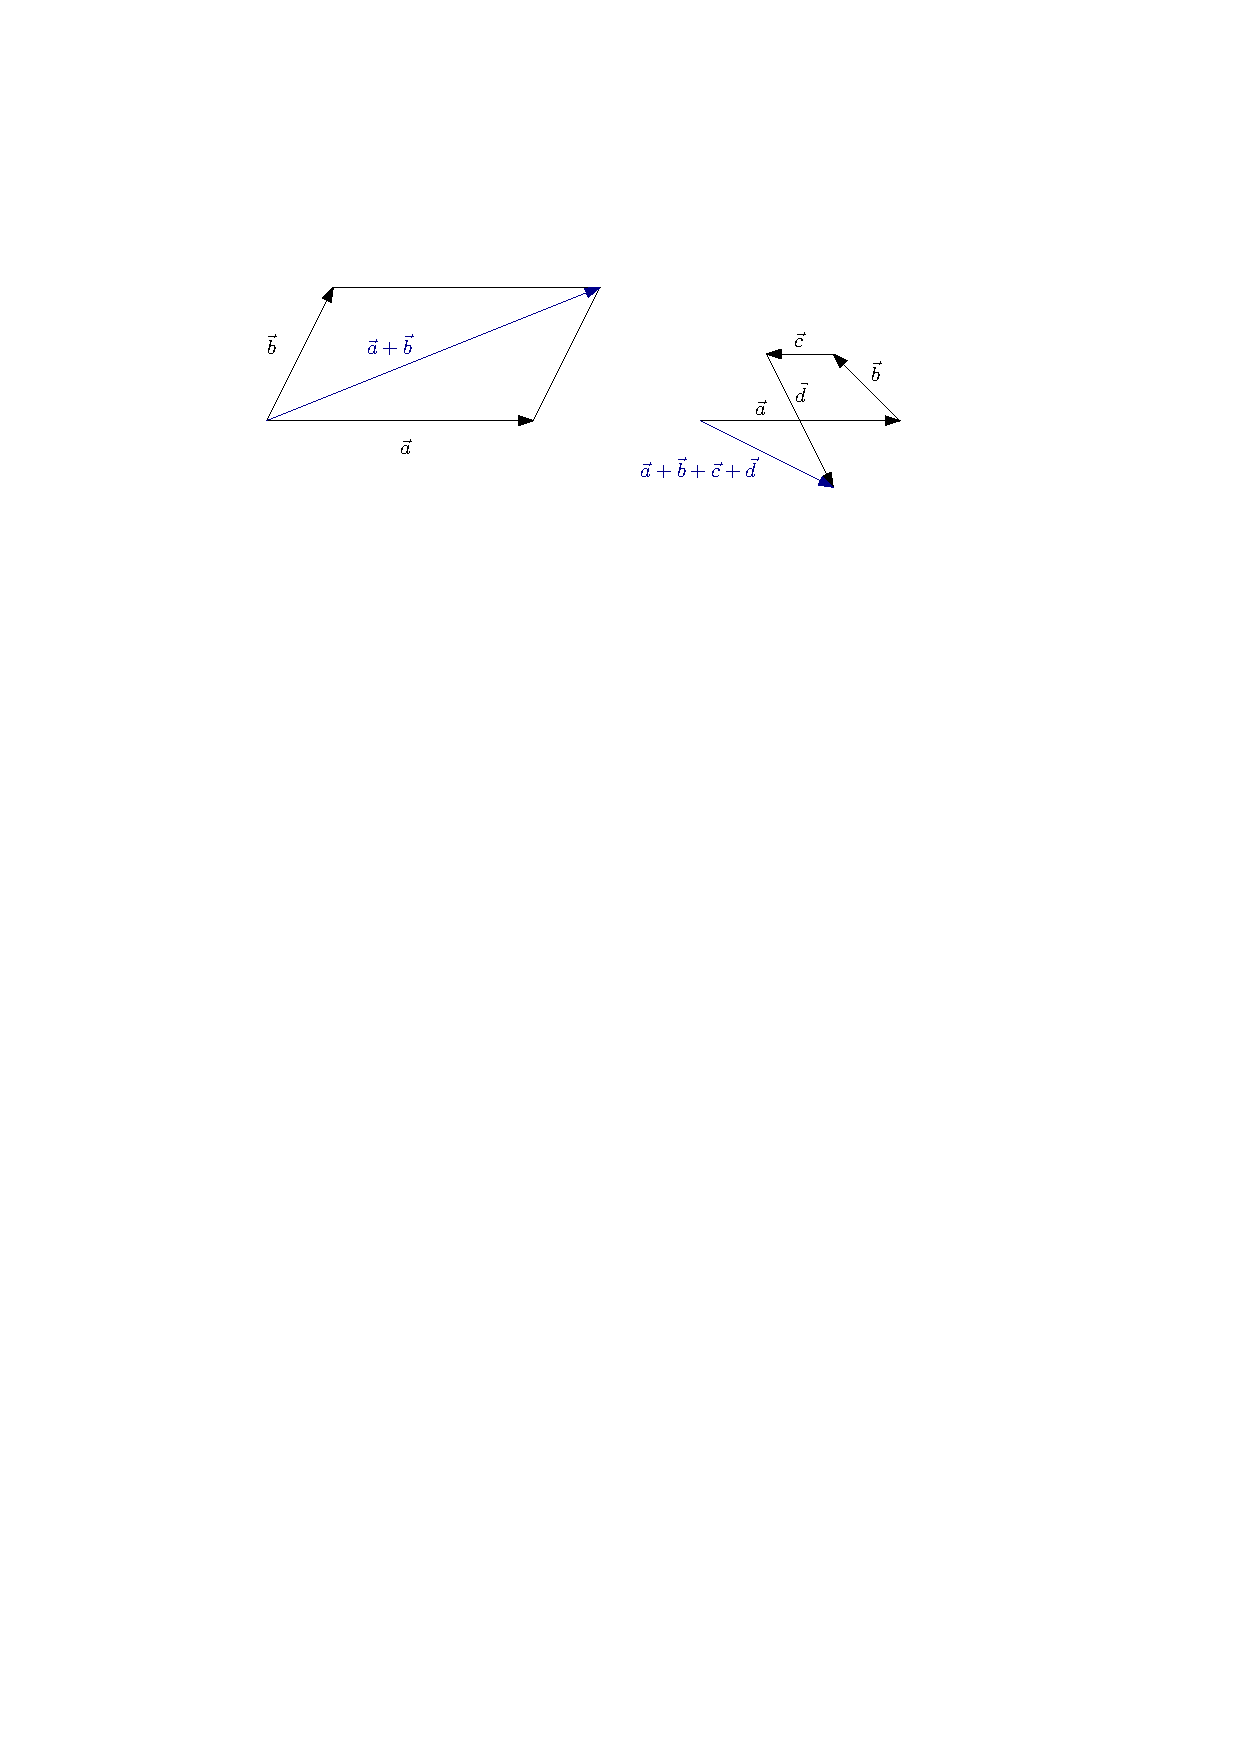
\includegraphics[width=0.7\textwidth]{sestevanje_vektorjev.pdf}
    \centering
\end{figure}

Ničelni vektor $\vec{0}=\vec{AA}=\vec{AB}+\vec{BA}$

Nasprotni vektor za $\vec{AB}$ je vektor $\vec{BA}$.

Enotski vektor je vektor z dolžino $1$.

Razlika vektorjev  je seštevanje nasprotnega vektorja.

\begin{zgled}
    V pravilnem šestkotniku $ABCDEF$, zapiši vse vektorje, ki so enaki $\vec{AB}$. Zapiši še vse nasprotne vektorje vektorja $\vec{SB}$, kjer je $S$ središče tega šestkotnika.
\end{zgled}

\begin{zgled}
    V kvadratu $ABCD$ izračunaj $\vec{BC}+\vec{CD}$, ter $\vec{DB}-\vec{CB}+\vec{CD}$.
\end{zgled}

\begin{zgled}
    V kocki $ABCDA'B'C'D'$ izračunaj vrednost izrazov $\vec{AD}+\vec{A'B'}$ in $\vec{AB}-\vec{D'A}-\vec{BB'}$.
\end{zgled}

\begin{zgled}
    Izračunaj $\vec{x}$, če je $\vec{x}-\vec{AC}=-\vec{AB}$.
\end{zgled}

\begin{example}
    DN 275b, 277bdf,  278e, 281ač. 283c
\end{example}

\subsubsection*{Množenje vektorja s številom (skalarjem)}

$m \cdot \vec{a}$, kjer $m\in\mathbb{R}_{\neq 0}$ je vektor z enako smerjo kot $\vec{a}$, usmerjenost je odvisna od predznaka $m$, njegova velikost pa je enaka $|m| \cdot |\vec{a}|$. Za $|m|>1$, se $\vec{a}$ podaljša, za $0<|m|<1$, se $\vec{a}$ skrajša.

\begin{enumerate}[i]
    \item Asociativnost v skalarnem delju: $m(n\vec{a})=(mn)\vec{a}$
    \item Distributivnost v vektorskem delu: $m(\vec{a}+\vec{b})=m\vec{a}+m\vec{b}$
    \item Distributivnost v skalarnem delu: $(m+n)\vec{a}=m\vec{a}+n\vec{a}$
\end{enumerate}

Iz vektorja $\vec{a}$ lahko naredimo enotski vektor $\vec{e}=\frac{\vec{a}}{|\vec{a}|}$

\begin{zgled}
    Izračunaj $n$, če za vektor $\vec{a}$ velja $(n^2 +3)\vec{a}-(n+2)\vec{a}=(3+n)\vec{a}+\vec{a}$.
\end{zgled}

\begin{zgled}
    Nariši trikotnik $ABC$, kjer $|\vec{AB}|=6cm$, $|\vec{BC}|=5cm$ in $|\vec{CA}|=3cm$. Nato nariši vektor $\vec{a}+2\vec{c}$.
\end{zgled}

\begin{example}
    DN 286b, 293ab
\end{example}

\section*{Odvisni in neodvisni vektorji}

Vektorja $\vec{a}$ in $\vec{b}$ sta \textbf{linearno odvisna}, če lahko enega izrazimo z drugim $\vec{a}=k\cdot \vec{b}$. Vektorja ležita na vzporednih nosilkah in rečemo, da sta kolinearna.

Dva vektorja $\vec{a}$ in $\vec{b}$ v ravnini, ki nista kolinearna sta \textbf{linearno neodvisna} in tvorita \textbf{bazo} ravnine. To pomeni, da lahko vsak vektor v ravnini na en sam način zapišemo kot njuno \textbf{linearno kombinacijo}:
\[\vec{v}=m\vec{a}+n\vec{b};\ m,n\in\mathbb{R}\]

\begin{figure}[H]
    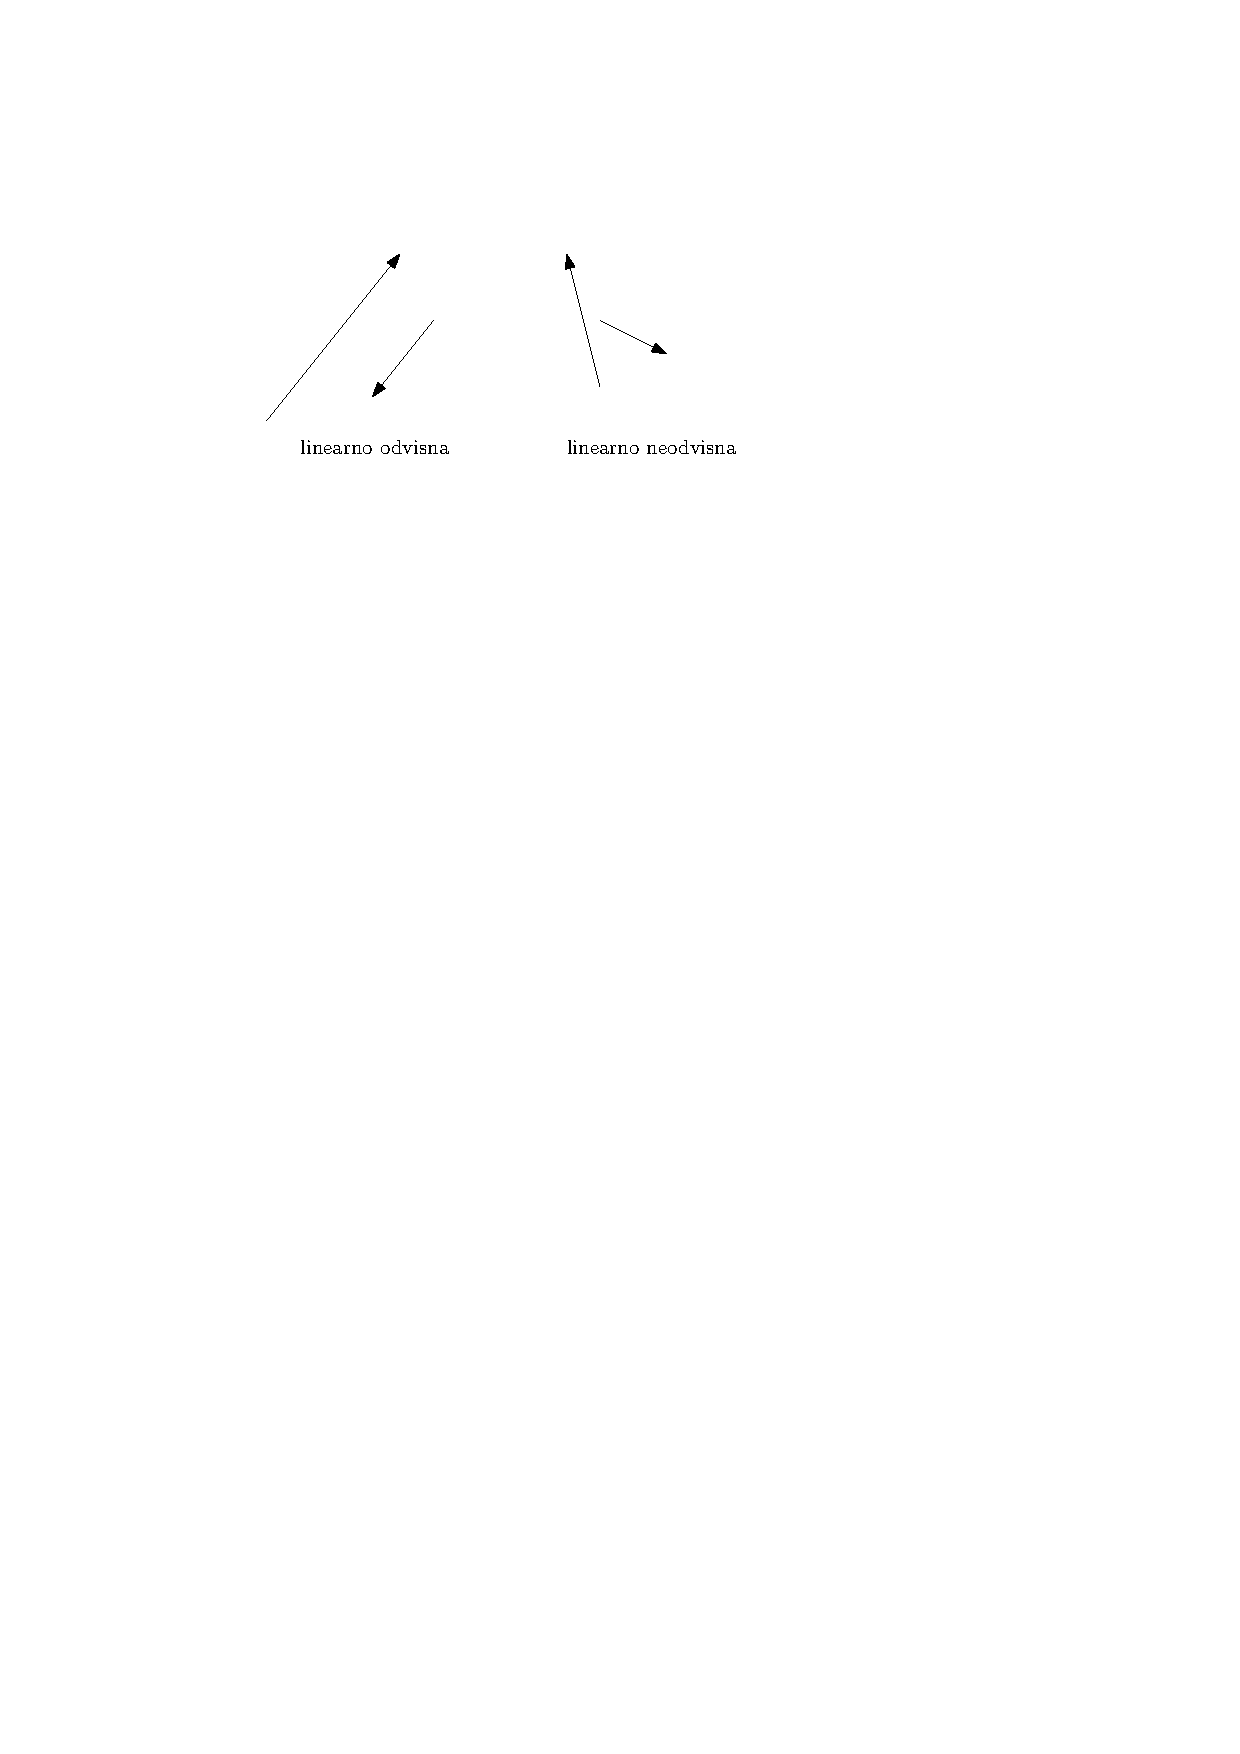
\includegraphics[width=0.5\textwidth]{odvisnost.pdf}
    \centering
\end{figure}

\begin{zgled}
    V pravokotniku $ABCD$ sta bazna vektorja $\vec{a}=\vec{AB}$ in $\vec{b}=\vec{AD}$. Točka $T_1$ je razpolovišče $CD$, točka $T_2$ pa deli stranico $AB$ v razmerju $|AT_2|:|T_2 B|=1:2$. Izrazi vektorje $\vec{T_2 C}$, $\vec{T_1 B}$ in $\vec{T_2 T_1}$ v bazi.
\end{zgled}

Vektorja $\vec{a}$ in $\vec{b}$ sta linearno neodvisna, če velja $m\vec{a}+n\vec{b}=0 \iff m=0=n$.

\begin{zgled}
    Za bazna vektorja $\vec{a}$ in $\vec{b}$ določi $m,n\in\mathbb{R}$, če velja $(n-2)(\vec{a}+\vec{b})=3(m\vec{a}+\vec{b})$.
\end{zgled}

\begin{zgled}
    V pravilnem šestkotniku $ABCDEF$ z bazo $\vec{a}=\vec{AB}$ in $\vec{b}=\vec{AF}$ zapiši vektorje $\vec{BF}$ in $\vec{AD}$.
\end{zgled}

\begin{zgled}
    V pravokotniku $ABCD$ je točka $N$ razpolovišče stranice $BC$, točka $M$ pa leži na stranici $AB$ tako, da $|AM|:|MB|=3:2$. V kakšnem razmerju deli stranica $MD$ daljico $AN$.
\end{zgled}

\begin{zgled}
    V paralelogramu $ABCD$, je $E$ na stranici $CD$, da $|DE|:|DC|=1:5$, točka $F$ pa je presek $BE$ in $AC$. Pokaži, da velja $\vec{EF}=\frac{4}{9}\vec{EB}$.
\end{zgled}

\begin{zgled}
    Pokaži, da težišče deli težiščnico v razmerju $2:1$.
\end{zgled}

\begin{example}
    DN 304, 311ac, 313, 314
\end{example}


\section{Vektorji v prostoru}

Bazo prostora sestavljajo trije neodvisni vektorji. Vsak vektor v prostoru lahko torej enolično zapišemo kot njihovo linearno kombinacijo.\\
Baza je ortogonalna, če so vektorji baze med sabo pravokotni. Baza je ortonormirana, če so vektorji pravokotni med sabo in dolžine $1$.\\
Standardna baza je ortonormirana baza $\{\vec{i},\vec{j},\vec{k}\}$, kjer ti vektorji ležijo zaporedno na poltrakih koordinatnih osi $x,y$ in $z$.\\
V tej standardni bazi , lahko vsako točko $A(a_1,a_2,a_3)$ predstavimo s krajevnim vektorjem $\vec{r_A}=a_1 \vec{i}+a_2\vec{j}+a_3\vec{k}$. Pišemo $\vec{r_A}=(a_1,a_2,a_3)$. Posebej $\vec{i}=(1,0,0) , \vec{j}=(0,1,0)$ in $\vec{k}=(0,0,1)$.

\begin{figure}[H]
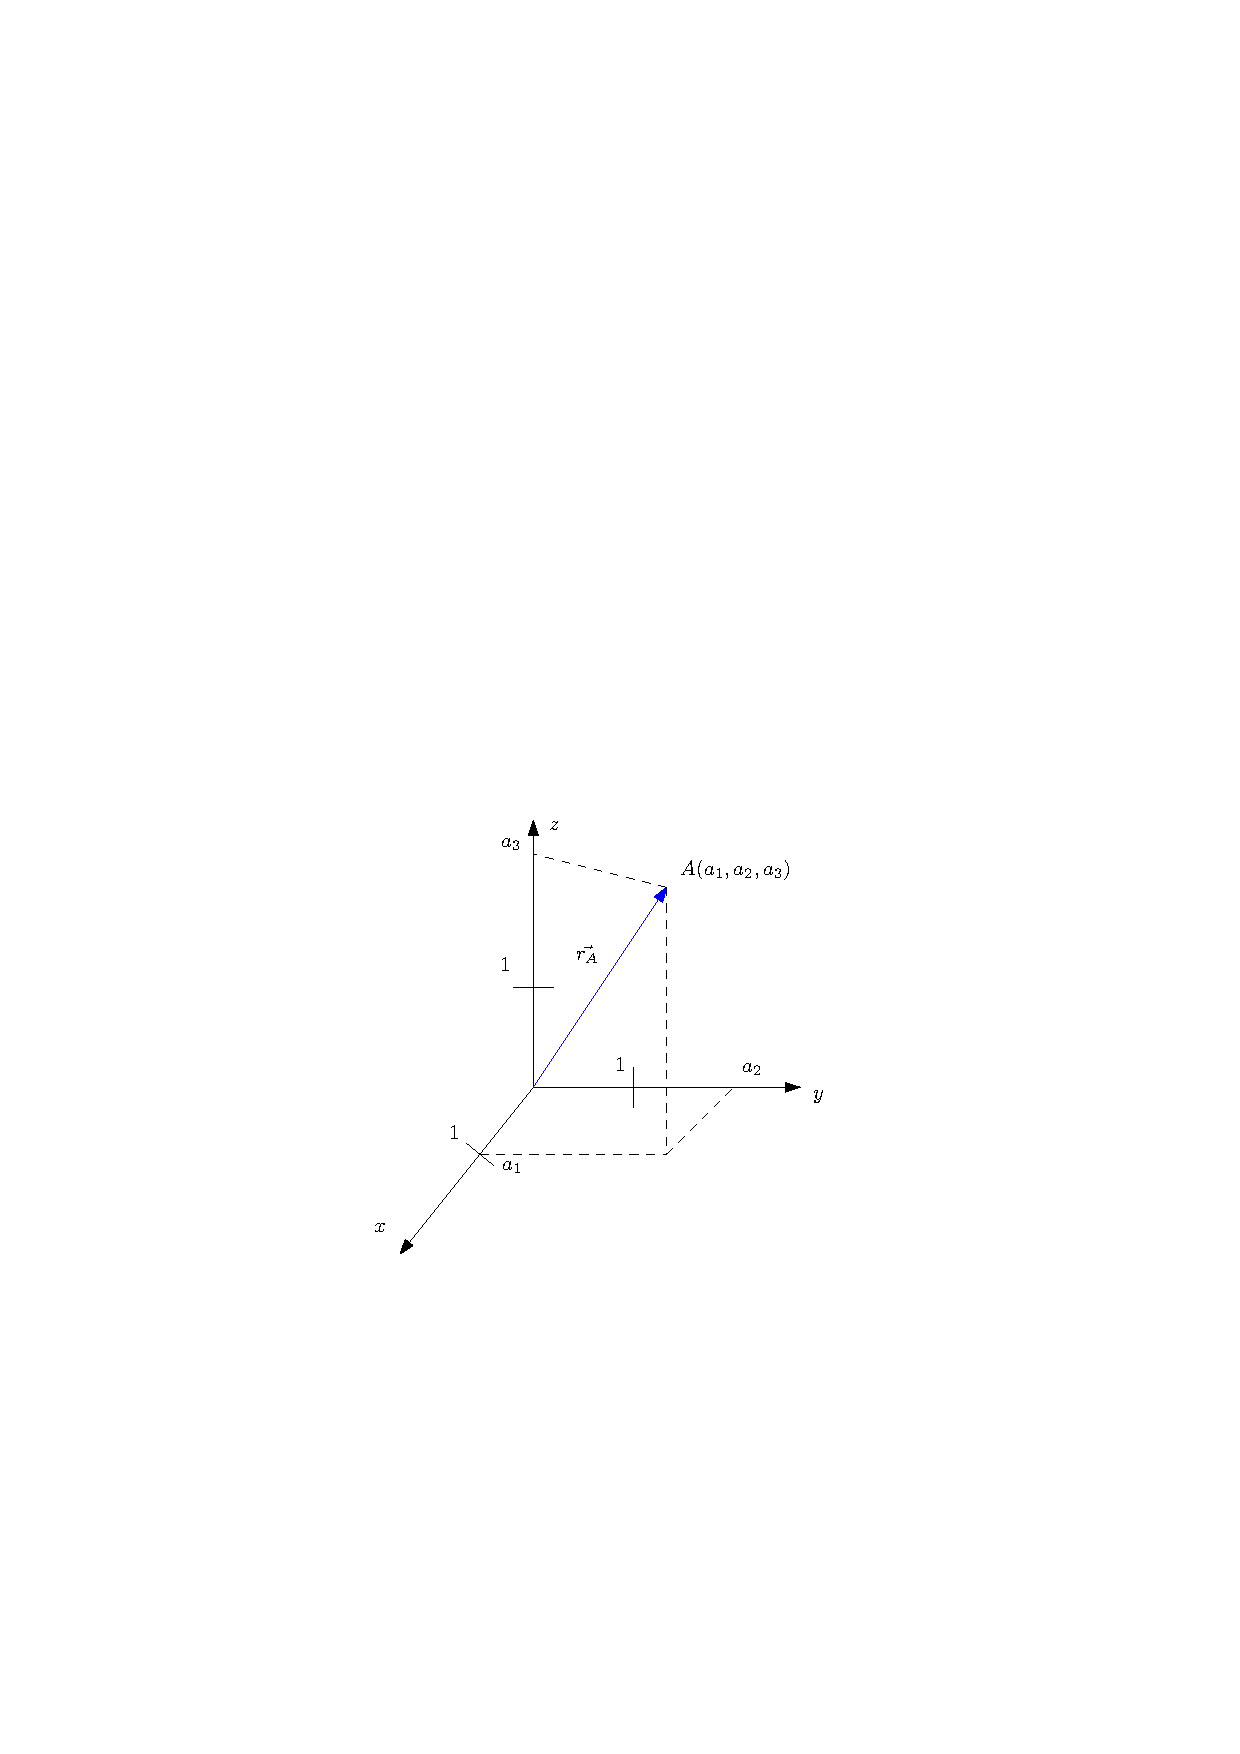
\includegraphics[width=0.7\textwidth]{vektorji_slika.pdf}
\centering
\end{figure}

\begin{zgled}
    Poiščimo eno ortogonalno in eno neoortogonalno bazo kocke.
\end{zgled}

\textbf{Računanje s krajevnimi vektorji:}

$(a_1,a_2,a_3)+(b_1,b_2,b_3)=(a_1+b_1,a_2+b_2,a_3+b_3)$\\
$n(a_1,a_2,a_3)=(na_1,na_2,na_3); n\in \mathbb{R}$

\begin{zgled}
    Zapišimo vektor daljice $AB$ in krajevni vektor razpolovišča te daljice. \href{https://youtu.be/KS_ZTJiAqdY}{Video rešitve}
\end{zgled}
\begin{zgled}
    Dani sta točki $A(-2,2,6)$ in $B(3,2,-4)$. Točka $T$ leži na daljici $AB$, da $|AT|:|TB|=4:1$. Izračunajmo koordinate $T$.
    \href{https://youtu.be/I5FE3vhoatk}{Video rešitve}
\end{zgled}

\begin{zgled}
    Dana sta vektorja $\vec{a}=(3,-2,0)$ in $\vec{b}=(-1,4,3)$. Zapišimo linearne kombinacije $\vec{a}+\vec{b}$ in $2\vec{a}-\frac{1}{2}\vec{b}$.
\end{zgled}

\begin{zgled}
    Določimo parameter $u$, da bosta vektorja $\vec{a}=(4,-6,u)$ in $\vec{b}=(-6,9,4)$ kolinearna. \href{https://youtu.be/bGx1agtOIvw}{Video rešitve}
\end{zgled}

\begin{zgled}
    Pokažimo, da so vektorji $\vec{a}=(1,-1,3), \vec{b}=(2,1,0)$ in $\vec{c}=(0,-3,6)$ koplanarni. \href{https://youtu.be/-qfYWHrmi-8}{Video rešitve}
\end{zgled}

Velja še, da je krajevni vektor $\vec{r_T}$ težišča $T$ trikotnika $ABC$ enak $\vec{r_T}=\frac{1}{3}(\vec{r_A}+\vec{r_B}+\vec{r_C})$.

\begin{example}
    NALOGE 321, 322, 324, 330, 340
\end{example}

\section{Skalarni produkt}

\[\vec{a}\cdot\vec{b}=|\vec{a}||\vec{b}|\cos\varphi, \ \text{kjer je}\  \varphi \ \text{vmesni kot}\]

Dolžina pravokotne projekcije $\vec{b}$ na $\vec{a}$ je $pr_{\vec{a}}\vec{b}=|\vec{b}|\cos\varphi$.\\

Za skalarni produkt velja komutativnost, distributivnost in homogenost.\\

$\vec{a} \perp\vec{b} \iff \vec{a}\cdot\vec{b}=0$\\

Dolžina vektorja $|\vec{a}|=\sqrt{\vec{a}\cdot\vec{a}}$\\

Kosinusni izrek $c^2=a^2+b^2-2ab\cos\gamma$

\begin{figure}[H]
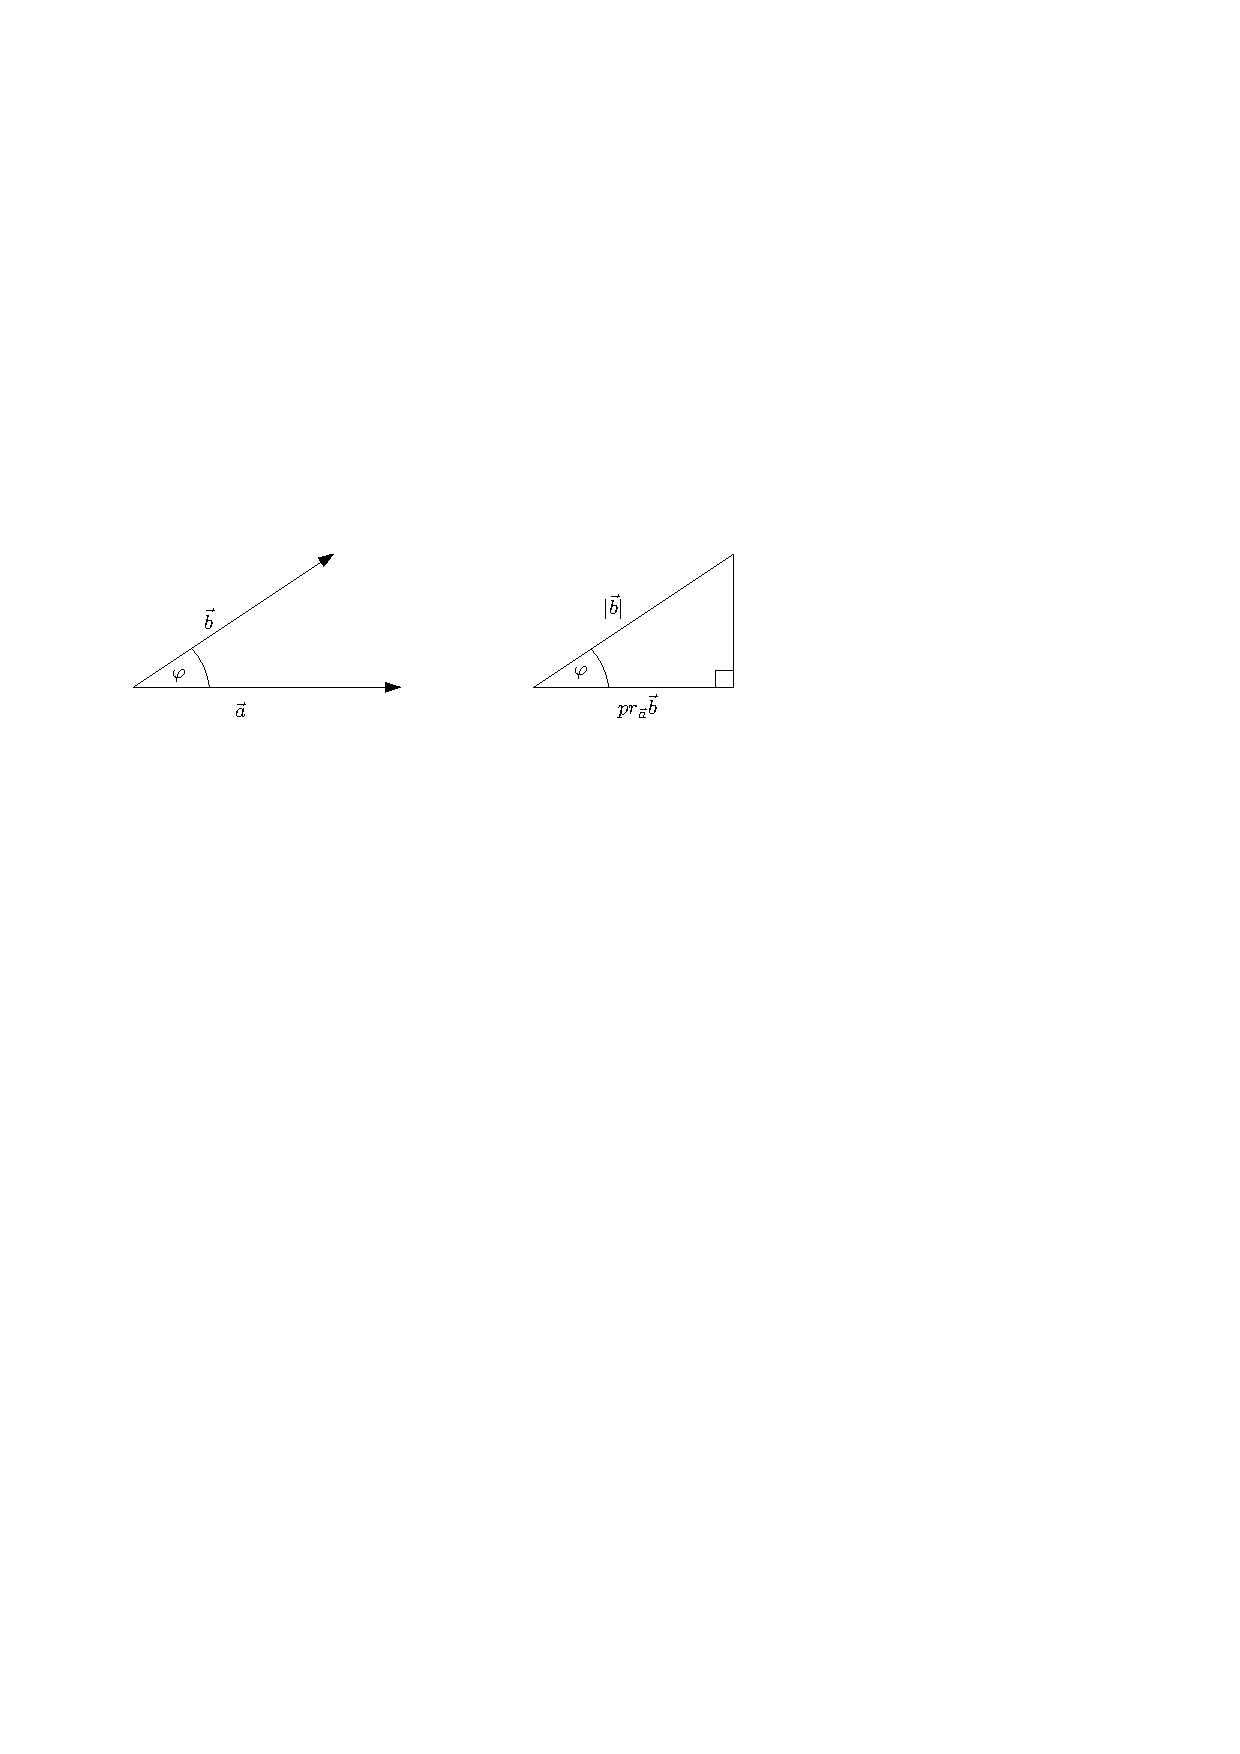
\includegraphics[width=0.7\textwidth]{skalarni.produkt.pdf}
\centering
\end{figure}

\begin{zgled}
    Izračunajmo dolžino vektorja $\vec{a}$, če ima $\vec{b}$ dolžino $6$, njun skalarni produkt je enak 21, njun vmesni kot pa $60^\circ$. Izračunajmo še $pr_{\vec{a}}\vec{b}$.
    \href{https://youtu.be/PCUppodHkyY}{Video rešitve}
\end{zgled}
\begin{zgled}
    Dolžina vektorja $\vec{a}$ je 3, $|\vec{b}|=4$, dolžina $2\vec{a}-\vec{b}$ pa $\sqrt{76}$. Izračunajmo kot med $\vec{a}$ in $\vec{b}$.
    \href{https://youtu.be/xMxlB981-ek}{Video rešitve}
\end{zgled}
\begin{zgled}
    V paralelogramu $ABCD$ je $a=7cm, b=4cm, \alpha=36^\circ$. Izračunajmo dolžino diagonale $f$.
    \href{https://youtu.be/cA2GKU8gsrw}{Video rešitve}
\end{zgled}

\begin{example}
    357a, 360c, 366 ampak izračunaj kot med a in b, 375ab, 377ab
\end{example}

\subsection{Skalarni produkt v ortonormirani bazi}

\[\vec{a}\cdot\vec{b}=a_1b_1+a_2b_2+a_3b_3\]
\[|\vec{a}|=\sqrt{a_1^2+a_2^2+a_3^2}\]
\[\cos\varphi=\frac{\vec{a}\cdot\vec{b}}{|\vec{a}||\vec{b}|}=\frac{a_1b_1+a_2b_2+a_3b_3}{\sqrt{a_1^2+a_2^2+a_3^2}\sqrt{b_1^2+b_2^2+b_3^2}}\]

\begin{zgled}
    Za vektorja $\vec{a}=(2,1,4)$ in $\vec{b}=(1,0,-1)$ izračunajmo $(2\vec{a}+\vec{b})\cdot\vec{b}$.
    \href{https://youtu.be/6Y_1Dqk4n-A}{Video rešitve}
\end{zgled}
\begin{zgled}
    Določimo komponento $u$, da bosta $\vec{a}=(-3,2u,5)$ in $\vec{b}=(6,u,2)$ pravokotna.
    \href{https://youtu.be/5CaojlnF_iI}{Video rešitve}
\end{zgled}
\begin{zgled}
    Naloga z mature 2021. \href{https://youtu.be/Qari4okAS7w}{Video rešitve}
\end{zgled}
    \begin{figure}[H]
    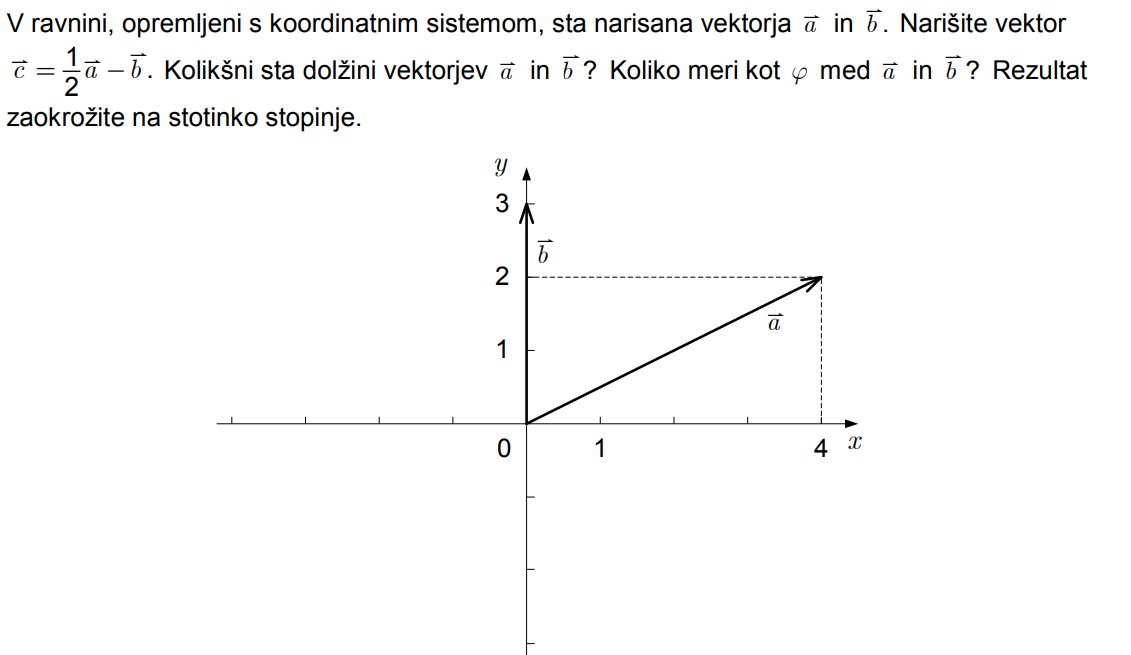
\includegraphics[width=\textwidth]{vektorji.naloga.png}
    \end{figure}

\begin{example}
    NALOGE 388 (razdalja=dolžina vektorja), 389 (enotski vektor=vektor/dolžina), 390ac, 393, 399, 405, 408, 414
\end{example}


\end{document}